% ------------------------------------------------------------------------------
% TYPO3 Versie 10.0 - What's New (English Version)
%
% @author	Michael Schams <schams.net>
% @license	Creative Commons BY-NC-SA 3.0
% @link		http://typo3.org/download/release-notes/whats-new/
% @language	Dutch
% ------------------------------------------------------------------------------

\section{Wijzigingen voor Ontwikkelaars}
\begin{frame}[fragile]
	\frametitle{Wijzigingen voor Ontwikkelaars}

	\begin{center}\huge{Hoofdstuk 4:}\end{center}
	\begin{center}\huge{\color{typo3darkgrey}\textbf{Wijzigingen voor Ontwikkelaars}}\end{center}

\end{frame}

% ------------------------------------------------------------------------------
% TYPO3 Versie 10.0 - Breaking Changes

\begin{frame}[fragile]
	\frametitle{Wijzigingen voor Integrators}
	\framesubtitle{Brekende wijzigingen}

	\small
		Let op ontwikkelaars: in TYPO3 v9 zijn PHP klassen, interfaces, klasse-aliassen,
		eigenschappen, functies, constantes, globale opties en variabelen, etc. als
		verouderd aangemerkt.

		\vspace{0.2cm}

		Volgens het TYPO3 \textbf{verouderingsbeleid}, zullen deze componenten verwijderd
		worden in TYPO3 v10.0.

		\vspace{0.2cm}

		Hieronder vallen ook enkele hooks, PHP bijschriften (zoals \texttt{@inject} en
		\texttt{@validate}), alsook wijzigingen in zichtbaarheid (bijv. van "\texttt{public}"
		in "\texttt{protected}".

		\vspace{0.2cm}

		Schakel de verouderingslog in, test code voorzichtig en bekijk de log om mogelijke
		problemen te vinden. Gebruik de ingebouwde
		\href{https://docs.typo3.org/m/typo3/reference-coreapi/master/en-us/ApiOverview/ExtensionScanner/Index.html}{Extensie-scanner}
		voor een overzicht van incompatibele code in extensies.

	\normalsize

\end{frame}

% ------------------------------------------------------------------------------
% Feature | 88643 | New Mail API based on symfony/mailer and symfony/mime
% Breaking | 88643 | Removed Swiftmailerswiftmailer Dependency

\begin{frame}[fragile]
	\frametitle{Wijzigingen voor Ontwikkelaars}
	\framesubtitle{Nieuwe E-mail-API}

	\begin{itemize}
		\item SwiftMailer is opgevolgd door modernere bibliotheken:

			\begin{itemize}
				\item \texttt{symfony/mime} voor het maken e-mailberichten
				\item \texttt{symfony/mailer} voor het versturen van e-mails
			\end{itemize}

		\item PHP functie \texttt{mail()} wordt niet langer ondersteund.

			\begin{itemize}\smaller
				\item[\ding{228}] Aangeraden wordt om \texttt{sendmail} of \texttt{smtp} te gebruiken.
			\end{itemize}\normalsize

		\item Maatwerk SwiftMailer plug-ins of transports vergen migratie.

		\item Zie de \href{https://symfony.com/doc/current/mailer.html}{Symfony Documentatie}
			voor meer details hoe de nieuwe E-mail API te gebruiken.
	\end{itemize}

\end{frame}

% ------------------------------------------------------------------------------
% Feature | 84112 | Symfony dependency injection for core and Extbase

\begin{frame}[fragile]
	\frametitle{Wijzigingen voor Ontwikkelaars}
	\framesubtitle{Symfony Dependency Management/Injection (1)}

	\begin{itemize}
		\item Het pakket \texttt{symfony/dependency-injection} is ge\"{\i}ntegreerd
			en wordt gebruikt om in het hele systeem afhankelijkheden te beheren en
			te injecteren in klassen.

		\item Met deze benadering moet uiteindelijk de Extbase injectiecontainer en
			en de objectbeheerder vervangen worden.

		\item Daarom moeten klassen aangepast worden en indien mogelijk vermeden:

			\begin{itemize}\small
				\item \texttt{\textbackslash
					TYPO3\textbackslash
					CMS\textbackslash
					Extbase\textbackslash
					Object\textbackslash
					ObjectManager}
				\item \texttt{\textbackslash
					TYPO3\textbackslash
					CMS\textbackslash
					Core\textbackslash
					Utility\textbackslash
					GeneralUtility::makeInstance()}
			\end{itemize}\normalsize

	\end{itemize}

\end{frame}

% ------------------------------------------------------------------------------
% Feature | 84112 | Symfony dependency injection for core and Extbase

\begin{frame}[fragile]
	\frametitle{Wijzigingen voor Ontwikkelaars}
	\framesubtitle{Symfony Dependency Management/Injection (2)}

	% decrease font size for code listing
	\lstset{basicstyle=\tiny\ttfamily}

	\begin{itemize}
		\item Configuratie-opties omvatten:

			\begin{itemize}
				\item Autobedrading (zie voorbeeld hieronder)
				\item Handmatige bedrading
					(zie \href{https://docs.typo3.org/c/typo3/cms-core/master/en-us/Changelog/10.0/Feature-84112-SymfonyDependencyInjectionForCoreAndExtbase.html}{lijst wijzigingen})
				\item Uitgebreide functionaliteit
					(zie \href{https://docs.typo3.org/c/typo3/cms-core/master/en-us/Changelog/10.0/Feature-84112-SymfonyDependencyInjectionForCoreAndExtbase.html}{lijst wijzigingen})
			\end{itemize}

		% \smaller Bijvoorbeeld "autobedrading":\normalsize

\begin{lstlisting}
# Configuration/Services.yaml
services:
  _defaults:
    autowire: true
    autoconfigure: true
    public: false

  Your\Namespace\:
    resource: '../Classes/*'
\end{lstlisting}

		\item Zie \href{https://symfony.com/doc/current/service_container.html}{Symfony documentatie} voor meer details.

	\end{itemize}

\end{frame}

% ------------------------------------------------------------------------------
% Feature | 88769 | Introduce a generic EventDispatcher based on PSR-14
% Feature | 88770 | Add PSR-14 EventDispatcher logic based on DI

\begin{frame}[fragile]
	\frametitle{Wijzigingen voor Ontwikkelaars}
	\framesubtitle{Afwikkeling gebeurtenissen (1)}

	\begin{itemize}
		\item Een nieuw systeem voor het afhandelen van gebeurtenissen is toegevoegd en zal
			de hooks en signal/slot concepten vervangen.

		\item Het is gebaseerd op de \href{https://www.php-fig.org/psr/psr-14}{PSR-14 standaard}
			waarmee ontwikkelaars op een simpele en consistente manier logica kunnen injecteren in een applicatie.

		\item PSR-14 bestaat uit de volgende vier onderdelen:

			\begin{itemize}
				\item Een \textbf{EventDispatcher} object waarmee je een gebeurtenis activeert.
				\item Een \textbf{ListenerProvider} object dat geregistreerde luisteraars voor alle gebeurtenissen bevat.
				\item Een of meerdere \textbf{Event} objecten die vanuit TYPO3 of extensies ("Emitter") aangeroepen worden.
				\item Een of meerdere \textbf{Listeners} (normaliter in extensies of PHP pakketten) die zijn geregistreerd.
			\end{itemize}

% Short-Term goal is to deprecate SignalSlot dispatcher in TYPO3 v10,
% and migrate all signals to the EventDispatcher.

	\end{itemize}

\end{frame}

% ------------------------------------------------------------------------------
% Feature | 88769 | Introduce a generic EventDispatcher based on PSR-14
% Feature | 88770 | Add PSR-14 EventDispatcher logic based on DI

\begin{frame}[fragile]
	\frametitle{Wijzigingen voor Ontwikkelaars}
	\framesubtitle{Afwikkeling gebeurtenissen (2)}

	% decrease font size for code listing
	\lstset{basicstyle=\tiny\ttfamily}

	Voorbeeld implementatie

	\begin{itemize}\smaller
		\item[\ding{202}] Voeg \texttt{event.listener} label toe aan bestand \texttt{Configuration/Services.yaml}:

\begin{lstlisting}
services:
  Vendor\Example\EventListener\NullMailer:
    tags:
      - { name: event.listener, identifier: 'myListener', event: TYPO3\CMS\Core\Mail\Event\AfterMailerInitializationEvent, before: 'redirects, anotherIdentifier' }
\end{lstlisting}

		\item[\ding{203}] Implementeer het event object:

\begin{lstlisting}
namespace Vendor\Example\EventListener;

class NullMailer
{
  public function __invoke(AfterMailerInitializationEvent $event): void
  {
    $event->getMailer()->injectMailSettings(['transport' => 'null']);
  }
}
\end{lstlisting}

	\end{itemize}\normalsize

\end{frame}

% ------------------------------------------------------------------------------
% Feature | 88769 | Introduce a generic EventDispatcher based on PSR-14
% Feature | 88770 | Add PSR-14 EventDispatcher logic based on DI

\begin{frame}[fragile]
	\frametitle{Wijzigingen voor Ontwikkelaars}
	\framesubtitle{Afwikkeling gebeurtenissen (3)}

	% decrease font size for code listing
	\lstset{basicstyle=\tiny\ttfamily}

	\begin{itemize}
		\item Lijst met beschikbare Event Listeners is beschikbaar in de backend:\newline
			\smaller
				(vereist systeemextensies \texttt{EXT:lowlevel})
			\normalsize
	\end{itemize}

	\begin{figure}
		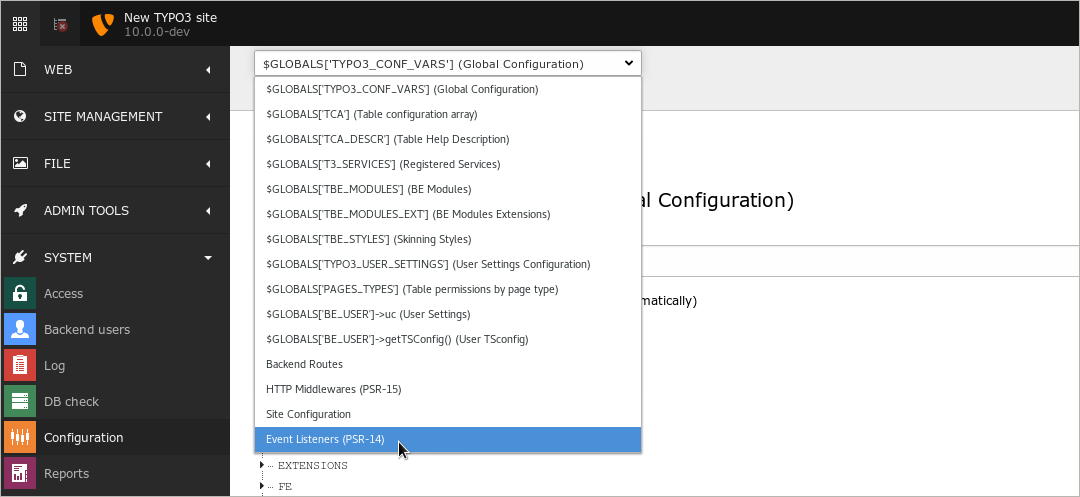
\includegraphics[width=0.70\linewidth]{ChangesForDevelopers/88770-PSR14-EventDispatcher.png}
	\end{figure}

\end{frame}


% ------------------------------------------------------------------------------
% Feature | 88769 | Introduce a generic EventDispatcher based on PSR-14
% Feature | 88770 | Add PSR-14 EventDispatcher logic based on DI

\begin{frame}[fragile]
	\frametitle{Wijzigingen voor Ontwikkelaars}
	\framesubtitle{Afwikkeling gebeurtenissen (4)}

	% decrease font size for code listing
	\lstset{basicstyle=\tiny\ttfamily}

	\begin{itemize}
		\item Aanbevolen methode:

			\begin{itemize}
				\item Voeg slechts één Listener per PHP klasse toe en gebruik \texttt{\_\_invoke()} als functienaam.
				\item Voeg "\texttt{Event}" achtervoegsel toe aan klassenaam bij een nieuwe Event klasse.
				\item Zet het Event PHP klassebestand in een geschikte map, bijv. \texttt{Classes/Database/Event}.
				\item Gebruik afhankelijkheidsinjectie in de vorm van een constructor-argument om indien nodig
					het EventDispatcher object te ontvangen.
			\end{itemize}

		\item Extra opmerking:\newline
			\small
				Gebeurtenissen die de TYPO3 core biedt volgen het beleid voor veroudering, behalve voor de constructor-argumenten
				die wel kunnen wijzigen.
			\normalsize

	\end{itemize}

\end{frame}

% ------------------------------------------------------------------------------
% Feature | 88799 | Use PSR-3 interface for logging

\begin{frame}[fragile]
	\frametitle{Wijzigingen voor Ontwikkelaars}
	\framesubtitle{PSR-3 koppelvlak voor logs}

	\begin{itemize}
		\item het TYPO3 Logging Framework (speciaal LogLevel en LogManager) gebruiken nu het
			\href{https://www.php-fig.org/psr/psr-3/}{PSR-3 Koppelvlak voor logs}.

		\item PSR-3 is een standaardmethode waarbij bibliotheken een
			\texttt{Psr\textbackslash
				Log\textbackslash
				LoggerInterface} object ontvangen en op een simpele en universele manier
				naar logs kunnen schrijven.

			\item Hiermee kunnen Ontwikkelaars eigen logs gebruiken en gebuik maken van
				andere logsystemen.

	\end{itemize}

\end{frame}

% ------------------------------------------------------------------------------
% Breaking | 88182 | jsfunc.inline.js has been dropped
% Breaking | 88427 | jsfunc.evalfield.js has been removed
% Breaking | 88667 | Removed additionalJavaScriptSubmit from FormEngine
% Deprecation | 88433 | Deprecate top.openUrlInWindow

\begin{frame}[fragile]
	\frametitle{Verouderde/verwijderde functies}
	\framesubtitle{JavaScript opties en functies (1)}

	\begin{itemize}
		\item De volgende JavaScript-bestanden zijn verwijderd:

			\begin{itemize}
				\item \texttt{jsfunc.inline.js}
				\item \texttt{jsfunc.evalfield.js}
			\end{itemize}

			\begin{itemize}\smaller
				\item[\ding{228}] Gebruik \texttt{TYPO3/CMS/Backend/FormEngineValidation} in plaats daarvan.
			\end{itemize}\normalsize

		\item Extra submit-handlers kunnen voorheen zijn toegevoegd met de optie \texttt{additionalJavaScriptSubmit}.
			Deze optie is verwijderd.

			\begin{itemize}\smaller
				\item[\ding{228}] Maak en registreer in plaats hiervan een AMD module.
			\end{itemize}\normalsize

		\item De globale JavaScript-functie \texttt{top.openUrlInWindow()} is als verouderd aangemerkt.

	\end{itemize}

\end{frame}

% ------------------------------------------------------------------------------
% Breaking | 88411 | TBE_EDITOR.typo3form removed
% Deprecation | 88432 | Replaced md5js with an AMD module
% Deprecation | 88428 | top.rawurlencode and top.str_replace
% Deprecation | 88651 | Replace TYPO3/CMS/Backend/SplitButtons with TYPO3/CMS/Backend/DocumentSaveActions

\begin{frame}[fragile]
	\frametitle{Verouderde/verwijderde functies}
	\framesubtitle{JavaScript opties en functies (2)}

	\begin{itemize}

		\item Het globale object \texttt{TBE\_EDITOR.typo3form} en z'n achterliggende lagen \texttt{typo3FormFieldSet}
			en \texttt{typo3FormFieldGet} zijn verwijderd.

		\item Bestand \texttt{md5.js} is als verouderd aangemerkt.

			\begin{itemize}\smaller
				\item[\ding{228}] Laad in plaats hiervan de AMD module \texttt{TYPO3/CMS/Backend/Hashing/Md5} via RequireJS.
			\end{itemize}\normalsize

		\item De volgende globale JavaScript-functies zijn als verouderd aangemerkt:

		\begin{itemize}
			\item \texttt{top.rawurlencode()}
			\item \texttt{top.str\_replace()}
		\end{itemize}

		\item Module \texttt{TYPO3/CMS/Backend.SplitButtons} is als verouderd aangemerkt.

			\begin{itemize}\smaller
				\item[\ding{228}] Gebruik in plaats hiervan \texttt{TYPO3/CMS/Backend/DocumentSaveActions}.
			\end{itemize}\normalsize

 	\end{itemize}

\end{frame}

% ------------------------------------------------------------------------------
% Important | 87894 | Removed PHP Dependency algo26-matthiasidna-convert

\begin{frame}[fragile]
	\frametitle{Wijzigingen voor Ontwikkelaars}
	\framesubtitle{UTF-8-gebaseerde domeinen}

	\begin{itemize}
		\item PHP heeft eigen functies om domeinen van UTF-8 naar IDNA ASCII formaat (“punicode”) om te zetten,
			bijv. \href{https://www.php.net/manual/en/function.idn-to-ascii.php}{idn\_to\_ascii()}.

		\item Deze kunnen direct gebruikt worden als de PHP extensie
			"\href{https://www.php.net/manual/en/book.intl.php}{intl}" aanwezig is.

		\item Als de PHP extensie niet aanwezig is biedt het pakket \texttt{symfony/polyfill-intl-idn}
			nu de functies.

		\item Hiervoor werd het pakket \texttt{algo26-matthias/idna-convert} gebruikt en deze is nu verwijderd.

	\end{itemize}

\end{frame}

% ------------------------------------------------------------------------------
% Feature | 87665 | Introduce BitSet class

\begin{frame}[fragile]
	\frametitle{Wijzigingen voor Ontwikkelaars}
	\framesubtitle{BitSet Class}

	% decrease font size for code listing
	\lstset{basicstyle=\tiny\ttfamily}

	\begin{itemize}
		\item Een nieuwe klasse is beschikbaar voor het efficiënt gebruiken van booleaanse vlaggen:\newline

			\texttt{TYPO3\textbackslash
				CMS\textbackslash
				Core\textbackslash
				Type\textbackslash
				BitSet}

		\item Bijvoorbeeld:

\begin{lstlisting}
define('PERMISSIONS_NONE', 0b0); // 0
define('PERMISSIONS_PAGE_SHOW', 0b1); // 1
define('PERMISSIONS_PAGE_EDIT', 0b10); // 2
define('PERMISSIONS_PAGE_DELETE', 0b100); // 4
define('PERMISSIONS_PAGE_NEW', 0b1000); // 8
define('PERMISSIONS_CONTENT_EDIT', 0b10000); // 16
define('PERMISSIONS_ALL', 0b11111); // 31

$bitSet = new \TYPO3\CMS\Core\Type\BitSet(PERMISSIONS_PAGE_SHOW | PERMISSIONS_PAGE_NEW);
$bitSet->get(PERMISSIONS_PAGE_SHOW); // true
$bitSet->get(PERMISSIONS_CONTENT_EDIT); // false
\end{lstlisting}

	\end{itemize}

\end{frame}

% ------------------------------------------------------------------------------
% Important | 87516 | Remove Core HTTP Request Handler Interface

\begin{frame}[fragile]
	\frametitle{Wijzigingen voor Ontwikkelaars}
	\framesubtitle{Request Handler (1)}

	\begin{itemize}
		\item Het volgende interne koppelvlak is verwijderd en vervangen door
			koppelvlakken van PSR-15 request handler en middleware:\newline
			\texttt{TYPO3\textbackslash
				CMS\textbackslash
				Core\textbackslash
				Http\textbackslash
				RequestHandlerInterface}

	\end{itemize}

\end{frame}

% ------------------------------------------------------------------------------
% Breaking | 88687 | Configure extbase request handlers via PHP

\begin{frame}[fragile]
	\frametitle{Wijzigingen voor Ontwikkelaars}
	\framesubtitle{Request Handler (2)}

	% decrease font size for code listing
	\lstset{basicstyle=\tiny\ttfamily}

	\begin{itemize}
		\item De configuratie van Extbase request handlers is niet langer mogelijk met TypoScript.

		\smaller\textbf{Oude} methode in TypoScript:\normalsize
\begin{lstlisting}
config.tx_extbase {
  mvc {
    requestHandlers {
      Vendor\Example\Mvc\Web\FrontendRequestHandler = Vendor\Example\Mvc\Web\FrontendRequestHandler
    }
  }
}
\end{lstlisting}

		\smaller\textbf{Nieuwe} methode in bestand \texttt{Configuration/Extbase/RequestHandlers.php}:\normalsize
\begin{lstlisting}
<?php
declare(strict_types = 1);

return [
  \Vendor\Example\Mvc\Web\FrontendRequestHandler::class,
];
\end{lstlisting}

	\end{itemize}

\end{frame}


% ------------------------------------------------------------------------------
% Deprecation | 88366 | Default caching framework cache names changed

\begin{frame}[fragile]
	\frametitle{Wijzigingen voor Ontwikkelaars}
	\framesubtitle{Caching Framework}

	% decrease font size for code listing
	\lstset{basicstyle=\tiny\ttfamily}

	\begin{itemize}
		\item De volgende caches zijn hernoemd:

			\begin{itemize}\smaller
				\item \texttt{cache\_core} \textrightarrow\hspace{0.1cm}\texttt{core}
				\item \texttt{cache\_hash} \textrightarrow\hspace{0.1cm}\texttt{hash}
				\item \texttt{cache\_pages} \textrightarrow\hspace{0.1cm}\texttt{pages}
				\item \texttt{cache\_pagesection} \textrightarrow\hspace{0.1cm}\texttt{pagesection}
				\item \texttt{cache\_runtime} \textrightarrow\hspace{0.1cm}\texttt{runtime}
				\item \texttt{cache\_rootline} \textrightarrow\hspace{0.1cm}\texttt{rootline}
				\item \texttt{cache\_imagesizes} \textrightarrow\hspace{0.1cm}\texttt{imagesizes}
			\end{itemize}\normalsize

		\item Nieuwe methode om de cache te benaderen:

\begin{lstlisting}
OUD:
$cacheManager->getCache('cache_core').

NIEUW:
$cacheManager->getCache('core')
\end{lstlisting}

		\item Het voorvoegsel \texttt{cf\_} is verwijderd uit de database tabellen.
	\end{itemize}

\end{frame}

% ------------------------------------------------------------------------------
% Deprecation | 87550 | Use controller classes when registering plugins/modules

\begin{frame}[fragile]
	\frametitle{Wijzigingen voor Ontwikkelaars}
	\framesubtitle{Extbase en Fluid}

	% decrease font size for code listing
	\lstset{basicstyle=\tiny\ttfamily}

	\begin{itemize}
		\item Het registreren van plug-ins/modules vergt nu volledige klassenamen

			\begin{itemize}\smaller
				\item \texttt{\textbackslash
					TYPO3\textbackslash
					CMS\textbackslash
					Extbase\textbackslash
					Utility\textbackslash
					ExtensionUtility::configurePlugin()}
				\item \texttt{\textbackslash
					TYPO3\textbackslash
					CMS\textbackslash
					Extbase\textbackslash
					Utility\textbackslash
					ExtensionUtility::registerModule()}
			\end{itemize}\normalsize

		\item Laat ook de vendor naam weg in de naam van de extensie (eerste argument).

			\begin{itemize}\smaller
				\item[\ding{228}] Gebruik "\texttt{ExampleBlog}" in plaats van "\texttt{Vendor.ExampleBlog}".
			\end{itemize}

		\item Bijvoorbeeld:

\begin{lstlisting}
\TYPO3\CMS\Extbase\Utility\ExtensionUtility::configurePlugin(
  'ExampleBlog', // previously: 'Vendor.ExampleBlog'
  'pi1',
  [
    \Vendor\Example\Controller\BlogController::class => 'list,update,delete'
  ],
  [
    \Vendor\Example\Controller\BlogController::class => 'list,update,delete'
  ]
);
\end{lstlisting}

	\end{itemize}

\end{frame}

% ------------------------------------------------------------------------------
% Breaking | 87627 | Remove Property extensionName of AbstractController

\begin{frame}[fragile]
	\frametitle{Verouderde/verwijderde functies}
	\framesubtitle{Extbase en Fluid}

	\begin{itemize}
		\item Eigenschap \texttt{extensionName} van AbstractController is verwijderd.

			\begin{itemize}\smaller
				\item[\ding{228}] Gebruik \texttt{\textbackslash
					TYPO3\textbackslash
					CMS\textbackslash
					Extbase\textbackslash
					Mvc\textbackslash
					Request::getControllerExtensionName()} in plaats daarvan.
			\end{itemize}\normalsize

	\end{itemize}

\end{frame}

% ------------------------------------------------------------------------------
% Feature | 87457 | Use symfony/propertyinfo to gather doc block information

\begin{frame}[fragile]
	\frametitle{Wijzigingen voor Ontwikkelaars}
	\framesubtitle{Extbase en Fluid}

	% decrease font size for code listing
	\lstset{basicstyle=\tiny\ttfamily}

	\begin{itemize}
		\item Extbase modellen ondersteunen nu afgekorte klassenamen in Doc-blokken.

\begin{lstlisting}
use TYPO3\CMS\Extbase\Persistence\ObjectStorage;
use ExtbaseTeam\BlogExample\Domain\Model\Comment;

class Post
{
  /**
   * @var ObjectStorage<Comment>
   */
  public $comments;
}
\end{lstlisting}

	\end{itemize}

\end{frame}

% ------------------------------------------------------------------------------
% Breaking | 87957 | Validators are not registered automatically in Extbase anymore

\begin{frame}[fragile]
	\frametitle{Wijzigingen voor Ontwikkelaars}
	\framesubtitle{Extbase en Fluid}

	% decrease font size for code listing
	\lstset{basicstyle=\tiny\ttfamily}

	\begin{itemize}
		\item Validators worden niet meer automatisch geregistreerd in Extbase.
		\item Voor een model met de naam
			\small\texttt{Vendor\textbackslash
				Example\textbackslash
				Domain\textbackslash
				Model\textbackslash
				Blog}\normalsize,\newline
			gebruikte Extbase automatisch de validator
			\small\texttt{Vendor\textbackslash
				Example\textbackslash
				Domain\textbackslash
				Validator\textbackslash
				BlogValidator}\normalsize

		\item Validators moeten nu handmatig geregistreerd worden:

\begin{lstlisting}
use Vendor\Example\Domain\Model\Blog;
use TYPO3\CMS\Extbase\Annotation as Extbase;
use TYPO3\CMS\Extbase\Mvc\Controller\ActionController;

class BlogController extends ActionController
{
  /**
   * @Extbase\Validate(param="blog", validator="Vendor\Example\Domain\Validator\BlogValidator")
   */
  public function showAction(Blog $blog)
  {
    // ...
  }
}
\end{lstlisting}

	\end{itemize}

\end{frame}

% ------------------------------------------------------------------------------
% Breaking | 87623 | Replace config.persistence.classes typoscript configuration (1)

\begin{frame}[fragile]
	\frametitle{Wijzigingen voor Ontwikkelaars}
	\framesubtitle{Extbase en Fluid - Mappen van klassen (1)}

	% decrease font size for code listing
	\lstset{basicstyle=\tiny\ttfamily}

	\begin{itemize}
		\item Het mappen van klassen met TypoScript voor opslag is niet langer ondersteund:

\begin{lstlisting}
config.tx_example_blog {
  persistence {
    classes {
      Vendor\Example\Domain\Model\Author {
        mapping {
          tableName = fe_users
          columns.name.mapOnProperty = fullname
        }
      }
    }
  }
}
\end{lstlisting}

	\end{itemize}

\end{frame}

% ------------------------------------------------------------------------------
% Breaking | 87623 | Replace config.persistence.classes typoscript configuration (2)

\begin{frame}[fragile]
	\frametitle{Wijzigingen voor Ontwikkelaars}
	\framesubtitle{Extbase en Fluid - Mappen van klassen (2)}

	% decrease font size for code listing
	\lstset{basicstyle=\tiny\ttfamily}

	\begin{itemize}
		\item Het mappen moet nu plaatsvinden in een PHP-bestand \texttt{Configuration/Extbase/Persistence/Classes.php}:

\begin{lstlisting}
<?php
declare(strict_types = 1);

return [
  \Vendor\Example\Domain\Model\Author::class => [
    'tableName' => 'fe_users',
    'properties' => [
      'name' => [
        'fieldName' => 'fullname'
      ]
    ]
  ]
];
\end{lstlisting}

	\end{itemize}

\end{frame}

% ------------------------------------------------------------------------------
% Breaking | 87594 | Harden Extbase

\begin{frame}[fragile]
	\frametitle{Wijzigingen voor Ontwikkelaars}
	\framesubtitle{Extbase en Fluid}

	% decrease font size for code listing
	\lstset{basicstyle=\smaller\ttfamily}

	\begin{itemize}
		\item Klassen gebruiken nu de "strict type" modus en type-hints voor scalaire parameters

\begin{lstlisting}
<?php
declare(strict_types=1);
\end{lstlisting}

		% Method signatures in Extbase classes have been updated.
		\item Dit geeft fatale PHP-fouten als de definitie van een functie in maatwerk
			extensies niet overeenkomt met interfaces en/of bovenliggende klassen.

		\item Zie \href{https://forge.typo3.org/issues/87594}{forge \#87594}
			voor een complete lijst van bestanden en hun wijzigingen.

		\item Dit is nog werk in uitvoering en verdere aanpassingen volgen.

	\end{itemize}

\end{frame}

% ------------------------------------------------------------------------------
% Breaking | 87937 | TCA option selicon_field_path removed
% Breaking | 87989 | TCA option setToDefaultOnCopy removed
% Breaking | 87936 | TCA for sys_history removed

\begin{frame}[fragile]
	\frametitle{Wijzigingen voor Ontwikkelaars}
	\framesubtitle{TCA wijzigingen}

	\begin{itemize}
		\item De volgende TCA opties zijn verwijderd:

			\begin{itemize}
				\item \texttt{\$TCA[\$tableName]['ctrl']['selicon\_field\_path']}
				\item \texttt{\$TCA[\$tableName]['ctrl']['setToDefaultOnCopy']}
			\end{itemize}

			\begin{itemize}\smaller
				\item[\ding{228}] Bij het kopiëren van records hoort een DataHandler velden terug te zetten.
			\end{itemize}\normalsize

		\item De hele TCA van \texttt{sys\_history} is verwijderen en het database-veld \texttt{pid} is verwijderd.
			Het benaderen van \texttt{\$GLOBALS['TCA']['sys\_history']} geeft nu een PHP waarschuwing.

	\end{itemize}

\end{frame}

% ------------------------------------------------------------------------------
% Breaking | 88527 | Overriding custom values in User Authentication derivatives

\begin{frame}[fragile]
	\frametitle{Wijzigingen voor Ontwikkelaars}
	\framesubtitle{Klassen/service voor gebruikersauthenticatie (1)}

	\begin{itemize}
		\item De volgende abstracte klasse is geherstructureerd:\newline
			\small\texttt{TYPO3\textbackslash
				CMS\textbackslash
				Core\textbackslash
				Authentication\textbackslash
				AbstractUserAuthentication}\normalsize
		\item Dit omvat ook de twee volgende directe onderklassen:

			\begin{itemize}
				\item \texttt{BackendUserAuthentication}
				\item \texttt{FrontendUserAuthentication}
			\end{itemize}

		\item De wijziging raakt de eigenschappen:

			\begin{itemize}
				\item \texttt{sessionTimeout}
				\item \texttt{gc\_time}
				\item \texttt{sessionDataLifetime}
				\item \texttt{loginType}
			\end{itemize}

	\end{itemize}

\end{frame}

% ------------------------------------------------------------------------------
% Breaking | 88646 | Removed inheritance of AbstractService from AbstractAuthenticationService

\begin{frame}[fragile]
	\frametitle{Wijzigingen voor Ontwikkelaars}
	\framesubtitle{Klassen/service voor gebruikersauthenticatie (2)}

	\begin{itemize}

		\item De volgende klasse overerft niet meer van
			\smaller\texttt{AbstractService}\normalsize\hspace{0.1cm}
			:
			\smaller\texttt{\textbackslash
				TYPO3\textbackslash
				CMS\textbackslash
				Core\textbackslash
				Authentication\textbackslash
				AbstractAuthenticationService}\normalsize

		\item Dit raakt mogelijk enkele beschikbare hooks en maatwerk authenticatie providers.

		\item Ontwikkelaars wordt aangeraden hun maatwerk authenticatieservices te controleren
			en indien nodig bij te werken.

	\end{itemize}

\end{frame}

% ------------------------------------------------------------------------------
% Deprecation | 87882 | File related controllers moved to EXT:filelist

\begin{frame}[fragile]
	\frametitle{Wijzigingen voor Ontwikkelaars}
	\framesubtitle{Controllers van Bestandslijst}

	\begin{itemize}
		\item De volgende controllers zijn verplaatst naar \texttt{EXT:filelist}:

			\begin{itemize}\small
				\item \texttt{CreateFolderController}
				\item \texttt{EditFileController}
				\item \texttt{FileUploadController}
				\item \texttt{RenameFileController}
				\item \texttt{ReplaceFileController}
			\end{itemize}\normalsize

		\item Als gevolg hiervan zijn de namespaces gewijzigd in\newline
			\texttt{\textbackslash
				TYPO3\textbackslash
				CMS\textbackslash
				Filelist\textbackslash
				Controller\textbackslash
				File}

		\vspace{0.2cm}

		\small
			Let op: Gebruik TYPO3 FAL als API en voeg eigen functionaliteit
			in eigen controllers in plaats van de bovenstaande \textbf{interne}
			controllers te hergebruiken.
		\normalsize

	\end{itemize}

\end{frame}

% ------------------------------------------------------------------------------
% Deprecation | 88499 | BackendUtility::getViewDomain()

\begin{frame}[fragile]
	\frametitle{Wijzigingen voor Ontwikkelaars}
	\framesubtitle{URL Frontend-voorvertoning}

	% decrease font size for code listing
	\lstset{basicstyle=\tiny\ttfamily}

	\begin{itemize}
		\item De volgende static functie is als verouderd aangemerkt:\newline
			\smaller\texttt{\textbackslash
				TYPO3\textbackslash
				CMS\textbackslash
				Backend\textbackslash
				Utility\textbackslash
				BackendUtility::getViewDomain()}\normalsize

		\item Vervang de functie door direct een site te detecteren op basis van de pagina ID binnen de TYPO3 backend.
		\item Bijvoorbeeld:

\begin{lstlisting}
$pageId = 123;
$site = GeneralUtility::makeInstance(SiteFinder::class)->getSiteByPageId($pageId);
$url = $site->getRouter()->generateUri($pageId, ['type' => 13]);
\end{lstlisting}

	\end{itemize}

\end{frame}

% ------------------------------------------------------------------------------
% Deprecation | 88406 | setCacheHash/noCacheHash options in ViewHelpers and UriBuilder

\begin{frame}[fragile]
	\frametitle{Wijzigingen voor Ontwikkelaars}
	\framesubtitle{cHash in UriBuilder en ViewHelpers}

	% decrease font size for code listing
	\lstset{basicstyle=\smaller\ttfamily}

	\begin{itemize}
		\item De volgende twee Extbase UriBuilder functies zijn als verouderd aangemerkt:

			\begin{itemize}
				\item \texttt{UriBuilder->setUseCacheHash()}
				\item \texttt{UriBuilder->getUseCacheHash()}
			\end{itemize}

		\item Dit heeft ook impact op een aantal Fluid ViewHelpers:
	\end{itemize}
	\vspace{-0.4cm}
	\begin{columns}[T]
		\begin{column}{.05\textwidth}
		\end{column}
		\begin{column}{.45\textwidth}
			\begin{itemize}\smaller
				\item \texttt{f:form}
				\item \texttt{f:link.action}
				\item \texttt{f:link.page}
				\item \texttt{f:link.typolink}
				\item \texttt{f:uri.action}
			\end{itemize}\normalsize
		\end{column}
		\begin{column}{.45\textwidth}
			\begin{itemize}\smaller
				\item \texttt{f:uri.page}
				\item \texttt{f:uri.typolink}
				\item \texttt{f:widget.link}
				\item \texttt{f:widget.uri}
			\end{itemize}\normalsize
		\end{column}
	\end{columns}
	\vspace{0.2cm}
	\begin{itemize}
		\item ... en ook de TypoLink opties "\texttt{useCacheHash}".
	\end{itemize}

\end{frame}

% ------------------------------------------------------------------------------
% Breaking | 88540 | Changed Request Workflow for Frontend Requests

\begin{frame}[fragile]
	\frametitle{Wijzigingen voor Ontwikkelaars}
	\framesubtitle{Frontend Request Afwikkeling}

	% decrease font size for code listing
	\lstset{basicstyle=\smaller\ttfamily}

	\begin{itemize}
		\item De afwikkeling van een frontend request is significant gewijzigd.

		\item De betrokken componenten zijn allen gebouwd als PSR-15 middlewares, de PSR-15 Request Handler,
			en de globale TypoScriptFrontendController (TSFE) sinds TYPO3 v9.

		\item Dit heeft impact op maatwerk code als de volgende hook en een frontend-sessie worden gebruikt:\newline
			{\fontsize{7}{8}\selectfont\texttt{\$GLOBALS['TYPO3\_CONF\_VARS']['SC\_OPTIONS']['tslib/class.tslib\_fe.php']['hook\_eofe']}}

			\begin{itemize}\smaller
				\item[\ding{228}] Gebruik een PSR-15 middleware in plaats van een hook of roep rechtstreeks
				\texttt{storeSessionData} aan binnen de hook.
			\end{itemize}\normalsize

	\end{itemize}

\end{frame}

% ------------------------------------------------------------------------------
% Breaking | 88498 | Global data for TimeTracker statistics removed

\begin{frame}[fragile]
	\frametitle{Wijzigingen voor Ontwikkelaars}
	\framesubtitle{Frontend Request Afwikkeling}

	% decrease font size for code listing
	\lstset{basicstyle=\smaller\ttfamily}

	\begin{itemize}
		\item De volgende globale variabelen zijn verwijderd:

			\begin{itemize}
				\item \texttt{\$GLOBALS['TYPO3\_MISC']['microtime\_start']}
				\item \texttt{\$GLOBALS['TYPO3\_MISC']['microtime\_end']}
				\item \texttt{\$GLOBALS['TYPO3\_MISC']['microtime\_BE\_USER\_start']}
				\item \texttt{\$GLOBALS['TYPO3\_MISC']['microtime\_BE\_USER\_end']}
			\end{itemize}

		\item De TYPO3 core gebruikte ze bijvoorbeeld in de Admin Panel en HTTP headers.

			\begin{itemize}\smaller
				\item[\ding{228}] Gebruik \texttt{TimeTracker->finish()} in plaats daarvan.
			\end{itemize}\normalsize

	\end{itemize}

\end{frame}


% ------------------------------------------------------------------------------
% Deprecation | 88569 | Locales::initialize() in favor of regular singleton instance
% Deprecation | 88473 | TypoScriptFrontendController->settingLocale

\begin{frame}[fragile]
	\frametitle{Verouderde/verwijderde functies}
	\framesubtitle{Locales}

	\begin{itemize}
		\item Functies \texttt{Locales::initialize()} is als verouderd aangemerkt.

			\begin{itemize}\smaller
				\item[\ding{228}] Gebruik \texttt{GeneralUtility::makeInstance(Locales::class)} of
				injecteer een afhankelijkheid om een instantie van de klasse \texttt{Locales} te krijgen.
			\end{itemize}\normalsize

		\item Functionaliteit van de volgende functie is als verouderd aangemerkt:\newline
			\texttt{TypoScriptFrontendController->settingLocale()}.

			\begin{itemize}\smaller
				\item[\ding{228}] Functie is nu beschikbaar als
				{\fontsize{8}{8} \selectfont \texttt{Locales::setSystemLocaleFromSiteLanguage()}.}
			\end{itemize}\normalsize

	\end{itemize}

\end{frame}

% ------------------------------------------------------------------------------
% Deprecation | 88559 | TSFE->sys_language_isocode

\begin{frame}[fragile]
	\frametitle{Verouderde/verwijderde functies}
	\framesubtitle{Locales}

	\begin{itemize}
		\item Publieke eigenschap \texttt{TypoScriptFrontendController->sys\_language\_isocode}
			is als verouderd gemarkeerd.

			\begin{itemize}\smaller
				\item[\ding{228}] Benader de eigenschap via \texttt{SiteLanguage->getTwoLetterIsoCode()}
				en \texttt{sitelanguage:twoLetterIsoCode} in plaats daarvan.
			\end{itemize}\normalsize

	\end{itemize}

\end{frame}

% ------------------------------------------------------------------------------
% Breaking | 88458 | Removed Frontend Track User ftu functionality

\begin{frame}[fragile]
	\frametitle{Verouderde/verwijderde functies}
	\framesubtitle{Frontend traceer gebruiker}

	\begin{itemize}

		\item De volgende publieke eigenschappen van klasse\newline
			\smaller\texttt{\textbackslash
				TYPO3\textbackslash
				CMS\textbackslash
				Core\textbackslash
				Authentication\textbackslash
				AbstractUserAuthentication}
			\normalsize\newline
			zijn verwijderd:

			\begin{itemize}\smaller
				\item \texttt{AbstractUserAuthentication->get\_name}
				\item \texttt{AbstractUserAuthentication->getFallBack}
				\item \texttt{AbstractUserAuthentication->getMethodEnabled}
				\item \texttt{AbstractUserAuthentication->get\_URL\_ID}
			\end{itemize}\normalsize

		\item Net als de eigenschap \texttt{getMethodUrlIdToken} van klasse\newline
			\smaller\texttt{\textbackslash
				TYPO3\textbackslash
				CMS\textbackslash
				Frontend\textbackslash
				Controller\textbackslash
				TypoScriptFrontendController}.
			\normalsize

		\item En de TypoScript optie \texttt{config.ftu},
			alsook de globale configuratie
			{\fontsize{8}{8} \selectfont \texttt{\$GLOBALS['TYPO3\_CONF\_VARS']['FE']['get\_url\_id\_token']}.}

	\end{itemize}

\end{frame}

% ------------------------------------------------------------------------------
% Breaking | 87305 | Use constructor injection in DataMapper

\begin{frame}[fragile]
	\frametitle{Verouderde/verwijderde functies}
	\framesubtitle{Constructor injectie in DataMapper}

	\begin{itemize}

		\item De volgende klasse gebruikt nu constructor-injectie in plaats van setter-injectie:
			\smaller
				\texttt{\textbackslash
					TYPO3\textbackslash
					CMS\textbackslash
					Extbase\textbackslash
					Persistence\textbackslash
					Generic\textbackslash
					Mapper\textbackslash
					DataMapper}
			\normalsize

			\begin{itemize}\smaller
				\item[\ding{228}] Vermijd \texttt{GeneralUtility::makeInstance()} en \texttt{ObjectManager->get()}.
				\item[\ding{228}] Gebruik afhankelijkheidsinjectie in plaats daarvan (bij voorkeur constructor-injectie).
			\end{itemize}\normalsize

	\end{itemize}

\end{frame}

% ------------------------------------------------------------------------------
% Feature | 88791 | Introduce PreviewAspect in Context

\begin{frame}[fragile]
	\frametitle{Verouderde/verwijderde functies}
	\framesubtitle{Context API}

	% decrease font size for code listing
	\lstset{basicstyle=\tiny\ttfamily}

	\begin{itemize}

		\item De Context API heeft een nieuw aspect "\texttt{frontend.preview}"
			die gebruikt kan worden om vast te stellen of de frontend in voorvertoningsmodus is:

\begin{lstlisting}
GeneralUtility::makeInstance(Context::class)
  ->getPropertyFromAspect('frontend.preview', 'isPreview');
\end{lstlisting}

		\item Dit aspect vervangt de volgende eigenschap die als verouderd is aangemerkt:
			\small\texttt{TypoScriptFrontendController->fePreview}\normalsize

	\end{itemize}

\end{frame}

% ------------------------------------------------------------------------------
% Feature | 88792 | Add TypoScriptAspect to handle TypoScript Rendering Context settings
% Deprecation | 88792 | forceTemplateParsing in TSFE and TemplateService has been deprecated

\begin{frame}[fragile]
	\frametitle{Verouderde/verwijderde functies}
	\framesubtitle{Context API}

	% decrease font size for code listing
	\lstset{basicstyle=\tiny\ttfamily}

	\begin{itemize}

		\item Een ander nieuw aspect \texttt{TypoScriptAspect} kan worden gebruikt om te zien/bewerken of
			TemplateRendering is geforceerd.

		\item De instelling \texttt{forceTemplateParsing} (TSFE en TemplateService) is als verouderd gemarkeerd.
			De context API kan in plaats daarvan gebruikt worden:

\begin{lstlisting}
GeneralUtility::makeInstance(Context::class)
  ->getPropertyFromAspect('typoscript', 'forcedTemplateParsing');

$context->setAspect(
  'typoscript',
  GeneralUtility::makeInstance(TypoScriptAspect::class, true)
);
\end{lstlisting}

	\end{itemize}

\end{frame}

% ------------------------------------------------------------------------------
% Breaking | 88525 | Remove “createDirs” directive of extension installation / ext_emconf.php
% Breaking | 87511 | Remove $viewFormatToObjectNameMap property
% Breaking | 87511 | Remove $namespacesViewObjectNamePattern property
% Feature | 87726 | Extend Frontend Login Controller Hook To Validate Password

\begin{frame}[fragile]
	\frametitle{Wijzigingen voor Ontwikkelaars}
	\framesubtitle{Diversen}

	\begin{itemize}
		\item Optie \texttt{createDirs} in bestand \texttt{ext\_emconf.php} wordt niet meer ondersteund.

			\begin{itemize}\smaller
				\item[\ding{228}] Mappen worden niet meer automatisch aangemaakt tijdens installatie van de extensie.
			\end{itemize}\normalsize

		\item De volgende twee eigenschappen in klasse
			\texttt{TYPO3\textbackslash
				CMS\textbackslash
				Extbase\textbackslash
				Mvc\textbackslash
				Controller\textbackslash
				ActionController}\newline
			zijn verwijderd:

			\begin{itemize}
				\item \texttt{\$namespacesViewObjectNamePattern}
				\item \texttt{\$viewFormatToObjectNameMap}
			\end{itemize}

		\item De volgende bestaande hook is uitgebreid en kan nu
			ook gebruikt worden om wachtwoorden te valideren:\newline
			{\fontsize{8}{10} \selectfont \texttt{\$GLOBALS['TYPO3\_CONF\_VARS']['EXTCONF']['felogin']['password\_changed']}}

	\end{itemize}

\end{frame}

% ------------------------------------------------------------------------------
% Deprecation | 87613 | Deprecate /TYPO3/CMS/Extbase/Utility/TypeHandlingUtility::hex2bin
% Deprecation | 88554 | Deprecated methods in VersionNumberUtility

\begin{frame}[fragile]
	\frametitle{Wijzigingen voor Ontwikkelaars}
	\framesubtitle{Diversen}

	\begin{itemize}

		\item De volgende functie is als verouderd aangemerkt:\newline
			\smaller\texttt{\textbackslash
				TYPO3\textbackslash
				CMS\textbackslash
				Extbase\textbackslash
				Utility\textbackslash
				TypeHandlingUtility::hex2bin()}\normalsize

			\begin{itemize}\smaller
				\item[\ding{228}] Gebruik de PHP functie \href{https://www.php.net/manual/en/function.hex2bin.php}{hex2bin()} in plaats hiervan.
			\end{itemize}\normalsize

		\item De volgende functies van klasse
			\smaller\texttt{\textbackslash
				TYPO3\textbackslash
				CMS\textbackslash
				Core\textbackslash
				Utility\textbackslash
				VersionNumberUtility}\normalsize\newline
			zijn als verouderderd aangemerkt:

			\begin{itemize}
				\item \texttt{convertIntegerToVersionNumber()}
				\item \texttt{splitVersionRange()}
				\item \texttt{raiseVersionNumber()}
			\end{itemize}

			\begin{itemize}\smaller
				\item[\ding{228}] Maak eigen functies hiervoor.
			\end{itemize}\normalsize

	\end{itemize}

\end{frame}

% ------------------------------------------------------------------------------
% Feature | 86964 | Allow getting class property default value
% Deprecation | 82669 | Streamline Backend route path inconsistencies

\begin{frame}[fragile]
	\frametitle{Wijzigingen voor Ontwikkelaars}
	\framesubtitle{Diversen}

	% decrease font size for code listing
	\lstset{basicstyle=\tiny\ttfamily}

	\begin{itemize}
		\item Het is nu mogelijk om de standaard waarde van een klasse-eigenschap
			te krijgen bij gebruik van de ReflectionService.

\begin{lstlisting}
$property = GeneralUtility::makeInstance(ReflectionService::class)
  ->getClassSchema(MyClass::class)
  ->getProperty('myProperty');
\end{lstlisting}

		\item Backend routes naar modules zonder pad-configuratie heten nu\newline
			standaard "\texttt{/module/<main-module>/<sub-module>}"\newline
			\small
				(voorbeeld: "\texttt{/module/web/ts}".)
			\normalsize

		\item Oude routes werken nog steeds (bijv. "\texttt{/web/ts/}") maar deze sytax zal verdwijnen in TYPO3 v11.

	\end{itemize}

\end{frame}

% ------------------------------------------------------------------------------
% Breaking | 88669 | FormEngine FormDataProvider parentPageTca removed
% Breaking | 88744 | Database fields related to CSS Styled Content removed
% Breaking | 88143 | Version-related database field “t3ver_id” removed
% Deprecation | 88746 | PageRepository PHP class moved from Frontend to Core Extension

\begin{frame}[fragile]
	\frametitle{Wijzigingen voor Ontwikkelaars}
	\framesubtitle{Diversen}

	\begin{itemize}
		\item De FormEngine DataProvider \texttt{parentPageTca} is verwijderd.

			\begin{itemize}\smaller
				\item[\ding{228}] Ontwikkelaars kunnen \texttt{\$GLOBALS['TCA']['pages']} direct gebruiken in plaats van \texttt{\$result['parentPageTca']}.
			\end{itemize}\normalsize

		\item De volgende database-velden zijn verwijderd:

			\begin{itemize}\smaller
				\item \texttt{tt\_content.spaceBefore} (vervangen door \texttt{space\_before\_class})
				\item \texttt{tt\_content.spaceAfter} (vervangen door \texttt{space\_after\_class})
				\item \texttt{pages.t3ver\_id} (ongebruikt sinds TYPO3 v9)
			\end{itemize}\normalsize

		\item De PHP klasse
			\texttt{\textbackslash
				TYPO3\textbackslash
				CMS\textbackslash
				Frontend\textbackslash
				Page\textbackslash
				PageRepository} is verplaatst van de "frontend" systeemextensie naar de core.

			\begin{itemize}\smaller
				\item Vervang door klasse:
					\texttt{\textbackslash
						TYPO3\textbackslash
						CMS\textbackslash
						Core\textbackslash
						Domain\textbackslash
						Repository\textbackslash
						PageRepository}
			\end{itemize}\normalsize

	\end{itemize}

\end{frame}

% ------------------------------------------------------------------------------
% Breaking | 88574 | 4th parameter of PageRepository>enableFields removed
% Deprecation | 85895 | Deprecate File::_getMetaData()
% Deprecation | 88662 | Deprecated backend route xMOD_tximpexp

\begin{frame}[fragile]
	\frametitle{Verouderde/verwijderde functies}
	\framesubtitle{Diversen}

	\begin{itemize}

		\item 4e parameter van functie \texttt{PageRepository->enableFields()} is verwijderd.

		\begin{itemize}\smaller
			\item[\ding{228}] Als 4e parameter gebruikt wordt met de waarde "\textbf{false}" kan dit veilig verwijderd worden.
			\item[\ding{228}] Als het gebruikt wordt met waarde "\textbf{true}" dan moet de code vervangen worden met een aparte instantie van \texttt{PageRepository} met een eigen \texttt{Context}.
		\end{itemize}\normalsize

		\item De interne functie \texttt{File::\_getMetaData()}, gebruikt voor het ophalen van metadata van een bestand,
			is als verouderd aangemerkt.

			\begin{itemize}\smaller
				\item[\ding{228}] Gebruik \texttt{\$fileObject->getMetaData()->get()} om nu de metadata op te halen.
			\end{itemize}\normalsize

		\item De route identifier "\texttt{xMOD\_tximpexp}" is als verouderd aangemerkt.

			\begin{itemize}\smaller
				\item[\ding{228}] Gebruik \texttt{tx\_impexp\_export} of \texttt{tx\_impexp\_import} afhankelijk van de situatie.
			\end{itemize}\normalsize

	\end{itemize}

\end{frame}

% ------------------------------------------------------------------------------
% Breaking | 88496 | Method getSwitchableControllerActions has been removed
% Breaking | 87567 | Global variable $TBE_TEMPLATE removed
% Breaking | 88660 | $GLOBALS[T3_VAR] removed

\begin{frame}[fragile]
	\frametitle{Verouderde/verwijderde functies}
	\framesubtitle{Diversen}

	\begin{itemize}

		\item De volgende abstracte functie is verwijderd:\newline
			\smaller
				\texttt{\textbackslash
					TYPO3\textbackslash
					CMS\textbackslash
					Extbase\textbackslash
					Configuration\textbackslash
					AbstractConfigurationManager::}\newline
					\texttt{getSwitchableControllerActions()}
			\normalsize

			\begin{itemize}\smaller
				\item[\ding{228}] Gebruik de nieuwe functienaam \texttt{getControllerConfiguration()} (zelfde PHP klasse).
			\end{itemize}\normalsize

		\item De globale variabele \texttt{\$TBE\_TEMPLATE} is verwijderd, inclusief
			de gerelateerde PSR-15 middeleware (die als intern was aangemerkt).

			\begin{itemize}\smaller
				\item[\ding{228}] Instantieer de DocumentTemplate klasse direct in de controller van de module.
				\item[\ding{228}] Migreer naar ModuleTemplate die sinds TYPO3 v7 beschikbaar is.
			\end{itemize}\normalsize

		\item De globale variabele \texttt{\$GLOBALS['T3\_VAR']} is verwijderd.\newline

	\end{itemize}

\end{frame}

% ------------------------------------------------------------------------------
